\documentclass[10pt]{article}
\usepackage[margin=1in]{geometry}
\usepackage[T1]{fontenc}
\usepackage{lmodern,microtype}
\usepackage{amsmath,booktabs,array,graphicx,longtable}
\usepackage{caption,placeins,url}
\usepackage[hidelinks]{hyperref}
\captionsetup{font=small,labelfont=bf}
\setlength{\emergencystretch}{2em}
\widowpenalty=10000
\clubpenalty=10000
\newcolumntype{L}[1]{>{\raggedright\arraybackslash}p{#1}}
\newcommand{\keeptablewithspace}[1]{\par\ifdim\dimexpr\pagegoal-\pagetotal\relax<#1\newpage\fi}
\renewcommand{\thetable}{S\arabic{table}}
\renewcommand{\thefigure}{S\arabic{figure}}
\title{Supplementary Material\\\large Environmental, temporal and source-information fusion for river DOC reconstruction}
\author{Zhaochen Yang}
\date{}
\begin{document}
\maketitle

\section{Task identity and reproduction}
This supplement accompanies the consolidated version-four manuscript. The work reuses completed model fits and saved predictions. The temporal, geographical and external tasks share the environmental--temporal--source architecture, with task-specific fitted states and validation fusion. Reconstruction scores use observed withheld cells. Full-grid outputs do not add observed truth or independent samples.

The two temporal roles contain 2,223 test cells at 69 stations and 1,778 cells at 67 stations. The internal geographical task contains 7,262 cells at 104 stations. Its separate fixed-query adaptation population contains 6,742 cells, excluding five designated support dates per station at every support count. The external task contains 6,514 primary cells at 130 stations and 5,864 fixed-query cells. Zero-support metrics for these two populations are distinct.

\begin{table}[!htbp]\centering\small
\caption{Saved model identities used in the three-procedure main comparison. Code names appear here only to locate the original products.}
\begin{tabular}{L{3.1cm}L{5.4cm}L{5.1cm}}\toprule
Procedure & Temporal prediction ID & Spatial/external prediction ID\\\midrule
Strong trees & \nolinkurl{station_hidden_trees} & \nolinkurl{station_hidden_trees}\\
Previous complete & \nolinkurl{upgraded_fusion} & \nolinkurl{unmonitored_integrated}\\
Current complete & \nolinkurl{available_fusion} & \nolinkurl{available_real_integrated}\\
Current native & \nolinkurl{available_native} & \nolinkurl{available_real_native}\\\bottomrule
\end{tabular}
\end{table}

Temporal experiment IDs are \nolinkurl{e2a_strict} and \nolinkurl{e2b_partial}, with seeds 42, 43 and 44. Spatial tasks use HUC4 1013, 1019, 0708, 1030 and 1101, with seeds 42--46. External deployment uses a fixed five-member mean. The source study directories are \nolinkurl{doc_current_source_temporal_v3_r1}, \nolinkurl{doc_current_availability_attention_geographical_v1} and \nolinkurl{doc_current_source_external_v2}, under \nolinkurl{experiments/phase4_transfer/}. The portable release is retained under \nolinkurl{doc_current_source_portable_v2_r1}.

\section{Training, information roles and preprocessing}
Environmental prediction uses log1p DOC as its fitting target and converts to concentration before native residual learning. Five station folds supply withheld-station reference predictions. The station-hidden fitting view removes the held fold's chemistry values and derived features. Donor references for a receiving fold exclude that receiving fold and the donor fold. These exclusions prevent a receiving training fold from contributing labels to its own experience bank.

The retained training procedure fits an observation-aware backbone with a 20-epoch cap, the daily native residual with a 120-epoch cap, and the station-hidden/source-attention correction with a 30-epoch cap. Early-stopping patience is five. The source-attention fit reuses the saved ecological and recurrent initialization of the preceding correction. Source-attention controls share that initialization and final training budget. Comparisons with older complete procedures include the accumulated recipe.

The encoder has hidden width 64 and ecological embedding width 32. The GRU uses twelve calendar months ending at the target month. The source operator uses twenty ecological candidates, two heads and 32 dimensions per head. A zero prior is always available. The local readout receives 38 retained features; three matched aggregate source descriptors extend this to 41 in the attention procedure. The source projection and residual readout are initialized to zero. Training-derived Q90 observations have weight two in the native absolute-error objective. Validation selects scale from zero, 0.25, 0.5 and one.

Dynamic and target statistics come from the permitted source training role. Historical static, coordinate and ecological preprocessing retains the development-cohort convention, which can use known unlabeled cohort covariates. It is saved and not re-estimated on external receiving sites. Daily descriptors are computed on the recorded discharge footprint, with availability represented explicitly. Same-month hydrology describes retrospective monthly reconstruction. No future month's inputs enter the twelve-month recurrent window.

Temporal inference permits train/context target observations and hides every validation/test target input. Spatial zero-support inference hides all local DOC, pH and conductivity, together with their values, masks, ages and derived support channels. Support adaptation opens only designated DOC observations after the zero-support prediction is fixed. Site-specific adjustment may use later support dates, so it is retrospective.

The temporal fusion family includes a log-affine concentration correction and environmental/native combinations. All six current temporal fits select log-affine fusion; seed 42 selects zero native scale in both tasks. Static ecological residual-memory blending is disabled in temporal tasks because training and validation stations overlap. It remains selectable, including zero weight, for spatial tasks. All five external deployment members select zero static-memory weight, so native and complete predictions coincide in that application.

\section{Detailed temporal and spatial metrics}
Metrics below reproduce the original point estimates. $R^2$ is computed inside each fitted task before averaging. Native residual and fused predictions are separate procedures. Previous versions and matched controls are retained without selecting different winners for different tasks.

\keeptablewithspace{18\baselineskip}
\begin{longtable}{L{7.2cm}rrrr}
\caption{Unobserved-period reconstruction; mean of three seeds. Errors and bias are in mg/L.}\\
\toprule Procedure & MAE & RMSE & $R^2$ & Bias\\\midrule\endfirsthead
\toprule Procedure & MAE & RMSE & $R^2$ & Bias\\\midrule\endhead
Current complete method & 0.785 & 1.222 & 0.599 & 0.139 \\
Current native residual & 0.896 & 1.329 & 0.525 & 0.440 \\
Context trees & 1.093 & 1.555 & 0.350 & 0.598 \\
Earlier complete fusion & 0.905 & 1.365 & 0.499 & 0.147 \\
Earlier native residual & 1.063 & 1.535 & 0.367 & 0.519 \\
Ordinary daily trees & 1.028 & 1.445 & 0.438 & 0.603 \\
Original hybrid & 0.875 & 1.333 & 0.522 & 0.140 \\
Strong environmental trees & 0.897 & 1.326 & 0.527 & 0.452 \\
Previous complete method & 0.786 & 1.223 & 0.598 & 0.138 \\
Previous native residual & 0.895 & 1.329 & 0.525 & 0.439 \\
\bottomrule

\end{longtable}

\keeptablewithspace{18\baselineskip}
\begin{longtable}{L{7.2cm}rrrr}
\caption{Observation-assisted-period reconstruction; mean of three seeds.}\\
\toprule Procedure & MAE & RMSE & $R^2$ & Bias\\\midrule\endfirsthead
\toprule Procedure & MAE & RMSE & $R^2$ & Bias\\\midrule\endhead
Current complete method & 0.797 & 1.208 & 0.601 & 0.241 \\
Current native residual & 0.935 & 1.344 & 0.506 & 0.551 \\
Context trees & 1.047 & 1.476 & 0.403 & 0.613 \\
Earlier complete fusion & 0.854 & 1.291 & 0.544 & 0.161 \\
Earlier native residual & 1.013 & 1.453 & 0.422 & 0.534 \\
Ordinary daily trees & 1.005 & 1.404 & 0.461 & 0.620 \\
Original hybrid & 0.807 & 1.261 & 0.565 & 0.111 \\
Strong environmental trees & 0.936 & 1.339 & 0.509 & 0.561 \\
Previous complete method & 0.798 & 1.209 & 0.600 & 0.241 \\
Previous native residual & 0.934 & 1.344 & 0.506 & 0.549 \\
\bottomrule

\end{longtable}

\begin{longtable}{L{7.2cm}rrrr}
\caption{Geographical zero-observation reconstruction; five seeds within region, five regions equally weighted.}\\
\toprule Procedure & MAE & RMSE & $R^2$ & Bias\\\midrule\endfirsthead
\toprule Procedure & MAE & RMSE & $R^2$ & Bias\\\midrule\endhead
Source anomaly attention / uniform / integrated & 2.273 & 3.851 & 0.138 & -0.650 \\
Source anomaly attention / uniform / native & 2.270 & 3.848 & 0.143 & -0.675 \\
Source anomaly attention / historical / integrated & 2.280 & 3.859 & 0.133 & -0.639 \\
Source anomaly attention / historical / native & 2.269 & 3.851 & 0.141 & -0.683 \\
Source anomaly attention / actual / integrated & 2.267 & 3.844 & 0.143 & -0.665 \\
Source anomaly attention / actual / native & 2.266 & 3.838 & 0.146 & -0.664 \\
Current complete method & 2.249 & 3.842 & 0.144 & -0.721 \\
Current native residual & 2.247 & 3.842 & 0.145 & -0.728 \\
Expanded current access / seasonal / integrated & 2.271 & 3.857 & 0.136 & -0.681 \\
Expanded current access / seasonal / native & 2.265 & 3.853 & 0.140 & -0.680 \\
Earlier full model & 2.360 & 3.894 & 0.133 & -0.490 \\
Source innovation / actual / integrated & 2.273 & 3.852 & 0.138 & -0.649 \\
Source innovation / actual / native & 2.268 & 3.845 & 0.144 & -0.667 \\
Aggregate-source trees & 2.315 & 3.870 & 0.124 & -0.560 \\
Full source innovation / uniform / integrated & 2.269 & 3.845 & 0.141 & -0.671 \\
Full source innovation / uniform / native & 2.256 & 3.835 & 0.148 & -0.672 \\
Full source innovation / historical / integrated & 2.284 & 3.868 & 0.129 & -0.664 \\
Full source innovation / historical / native & 2.277 & 3.864 & 0.135 & -0.691 \\
Full source innovation / actual / integrated & 2.266 & 3.844 & 0.142 & -0.675 \\
Full source innovation / actual / native & 2.265 & 3.844 & 0.143 & -0.694 \\
Full source innovation / seasonal / integrated & 2.274 & 3.860 & 0.133 & -0.670 \\
Full source innovation / seasonal / native & 2.263 & 3.854 & 0.141 & -0.696 \\
Ordinary daily trees & 2.441 & 3.921 & 0.109 & -0.309 \\
Relative source anomaly / uniform / integrated & 2.268 & 3.846 & 0.142 & -0.676 \\
Relative source anomaly / uniform / native & 2.259 & 3.837 & 0.147 & -0.670 \\
Relative source anomaly / historical / integrated & 2.276 & 3.858 & 0.135 & -0.648 \\
Relative source anomaly / historical / native & 2.262 & 3.847 & 0.143 & -0.677 \\
Relative source anomaly / actual / integrated & 2.258 & 3.837 & 0.147 & -0.656 \\
Relative source anomaly / actual / native & 2.260 & 3.832 & 0.148 & -0.651 \\
Strong environmental trees & 2.345 & 3.914 & 0.116 & -0.597 \\
Previous complete method & 2.282 & 3.865 & 0.131 & -0.649 \\
Previous native residual & 2.266 & 3.854 & 0.140 & -0.687 \\
\bottomrule

\end{longtable}

\keeptablewithspace{14\baselineskip}
\begin{longtable}{L{7.2cm}rrrr}
\caption{External all-observation metrics; error of fixed ensemble predictions.}\\
\toprule Procedure & MAE & RMSE & $R^2$ & Bias\\\midrule\endfirsthead
\toprule Procedure & MAE & RMSE & $R^2$ & Bias\\\midrule\endhead
Current complete method & 0.911 & 1.377 & -0.129 & -0.442 \\
Current native residual & 0.911 & 1.377 & -0.129 & -0.442 \\
Earlier full model & 0.984 & 1.428 & -0.214 & -0.411 \\
Ordinary daily trees & 0.837 & 1.238 & 0.087 & -0.038 \\
Strong environmental trees & 0.841 & 1.240 & 0.084 & -0.034 \\
Previous complete method & 0.915 & 1.378 & -0.130 & -0.434 \\
Previous native residual & 0.915 & 1.378 & -0.130 & -0.434 \\
\bottomrule

\end{longtable}

\section{Paired uncertainty and support curves}
The 5,000-draw station bootstrap retains all months and predictions of a station. Inside each draw, individual-seed errors are averaged, and geographical regions remain equally weighted. Seeds repeat the same ecological observations. A bootstrap draw with an empty geographical region is redrawn. Intervals describe uncertainty conditional on saved predictions and do not include refitting uncertainty. The external comparison uses ensemble predictions and a single regional population.

\begin{longtable}{L{2.7cm}L{6.4cm}rrr}
\caption{Main matched contrasts. Positive gain means lower MAE; interval bounds are in percentage points of relative reduction.}\\
\toprule Task & Comparison & Gain (\%) & Low & High\\\midrule\endfirsthead
\toprule Task & Comparison & Gain (\%) & Low & High\\\midrule\endhead
Unobserved periods & Current complete method vs Strong environmental trees & 12.506 & 8.701 & 15.912 \\
Unobserved periods & Current complete method vs Previous complete method & 0.107 & 0.011 & 0.199 \\
Unobserved periods & Current native residual vs Strong environmental trees & 0.075 & -0.511 & 0.654 \\
Observation-assisted periods & Current complete method vs Strong environmental trees & 14.882 & 11.855 & 17.612 \\
Observation-assisted periods & Current complete method vs Previous complete method & 0.086 & -0.013 & 0.188 \\
Observation-assisted periods & Current native residual vs Strong environmental trees & 0.112 & -0.517 & 0.775 \\
Unmonitored regions & Current complete method vs Strong environmental trees & 4.109 & 1.113 & 7.109 \\
Unmonitored regions & Current complete method vs Previous complete method & 1.478 & 0.416 & 2.672 \\
Unmonitored regions & Current complete method vs Expanded current access / seasonal / integrated & 0.968 & 0.455 & 1.547 \\
Unmonitored regions & Current complete method vs Full source innovation / actual / integrated & 0.781 & 0.282 & 1.341 \\
Unmonitored regions & Current complete method vs Relative source anomaly / actual / integrated & 0.432 & -0.259 & 1.271 \\
Unmonitored regions & Current native residual vs Expanded current access / seasonal / native & 0.796 & 0.202 & 1.516 \\
External application & Current complete method vs Strong environmental trees & -8.294 & -19.440 & 4.435 \\
External application & Current complete method vs Previous complete method & 0.483 & -0.393 & 1.560 \\
\bottomrule

\end{longtable}

Five support dates per eligible station follow the first, middle, last, first-quartile and third-quartile order. Nested prefixes define zero, one, three and five observations, with all five dates excluded from the query at every count. Adaptation uses a shrunken mean log residual, with shrinkage selected on source validation. One observation selects zero correction in the current external release. The model is not changed between support counts.

\begin{figure}[!htbp]\centering
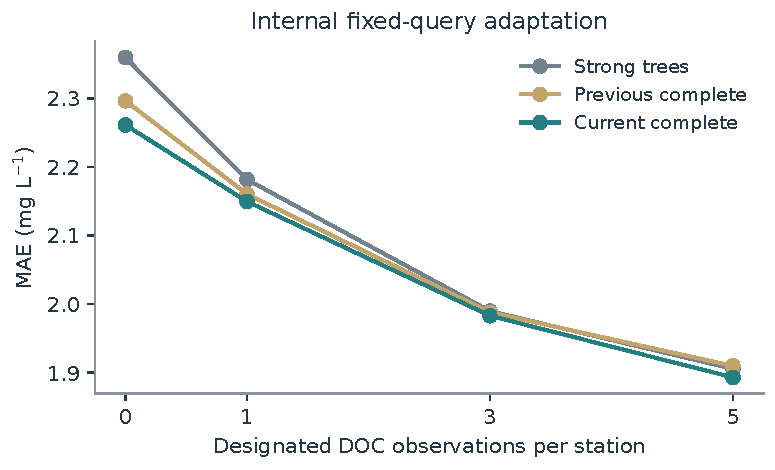
\includegraphics[width=.78\linewidth]{figures/spatiotemporal_v4/supp2_internal_support.pdf}
\caption{Internal adaptation on 6,742 fixed query cells. Five possible support dates per eligible station are excluded at every count. The curve's zero-observation population differs from the 7,262-cell primary result.}
\end{figure}

\section{High DOC, environmental strata and uncertainty}
Q90 thresholds are derived from source training labels separately for each task. The temporal tasks contain only twelve and seven unique high-DOC cells. Geographical regions contain 904, 43, 66, 15 and eleven cells, respectively; the last two are small tail populations. The external source-threshold tail has sixteen cells at eleven stations, and all compared tools miss these events. Repeated seeds do not increase these counts. Tail MAE and detection behavior are reported as separate quantities.

\begin{table}[!htbp]\centering\small
\caption{External station weighting, tail error and empirical intervals. Tail MAE uses sixteen unique cells. Coverage is in percent; concentration errors and widths are in mg/L.}
\begin{tabular}{L{5.3cm}rrrr}\toprule
Procedure & Station MAE & Q90 MAE & Coverage & Width\\\midrule
Current complete method & 0.821 & 9.578 & 83.27 & 2.737 \\
Strong environmental trees & 0.905 & 9.392 & 92.51 & 3.537 \\
Previous complete method & 0.841 & 9.566 & 84.92 & 2.889 \\
\bottomrule

\end{tabular}
\end{table}

Empirical 90\% intervals use a finite-rank source-validation quantile of absolute log1p error. Interval endpoints are transformed back to nonnegative concentration. Model selection and calibration share source validation, so no split-conformal guarantee is claimed. Adapted source-validation queries calibrate each support count. Current external coverage is 83.27\%, with median width 2.737~mg/L; at five supports it is 87.38\%, with width 2.397~mg/L.

\begin{figure}[!htbp]\centering
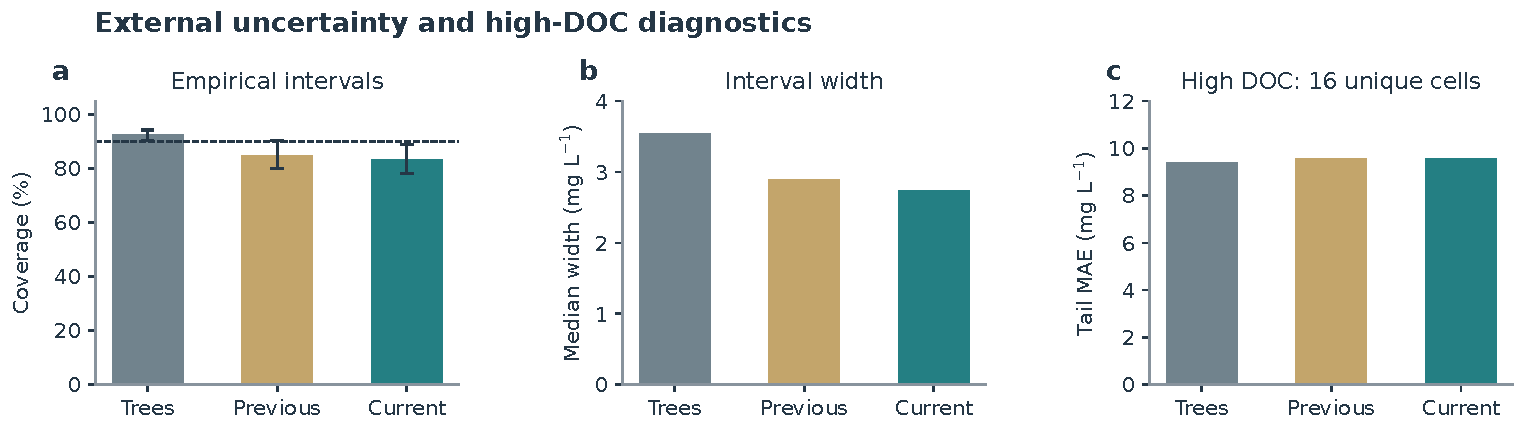
\includegraphics[width=\linewidth]{figures/spatiotemporal_v4/supp1_uncertainty_tail.pdf}
\caption{External empirical coverage, median width and upper-decile error. Coverage bars include station-bootstrap intervals; the dashed line denotes nominal 90\%. The narrow high-DOC population is explicitly reported.}
\end{figure}

Ecological novelty and nearest-source distance use training-derived ecological standardization and tertiles. Hydrological availability separates zero, one and two available monthly input channels. Geographical strata average usable region estimates, while external strata score the fixed ensemble. Empty external groups remain visible. These descriptive groups identify where reconstruction needs improvement without selecting a different predictor for each group.

\begin{figure}[!htbp]\centering
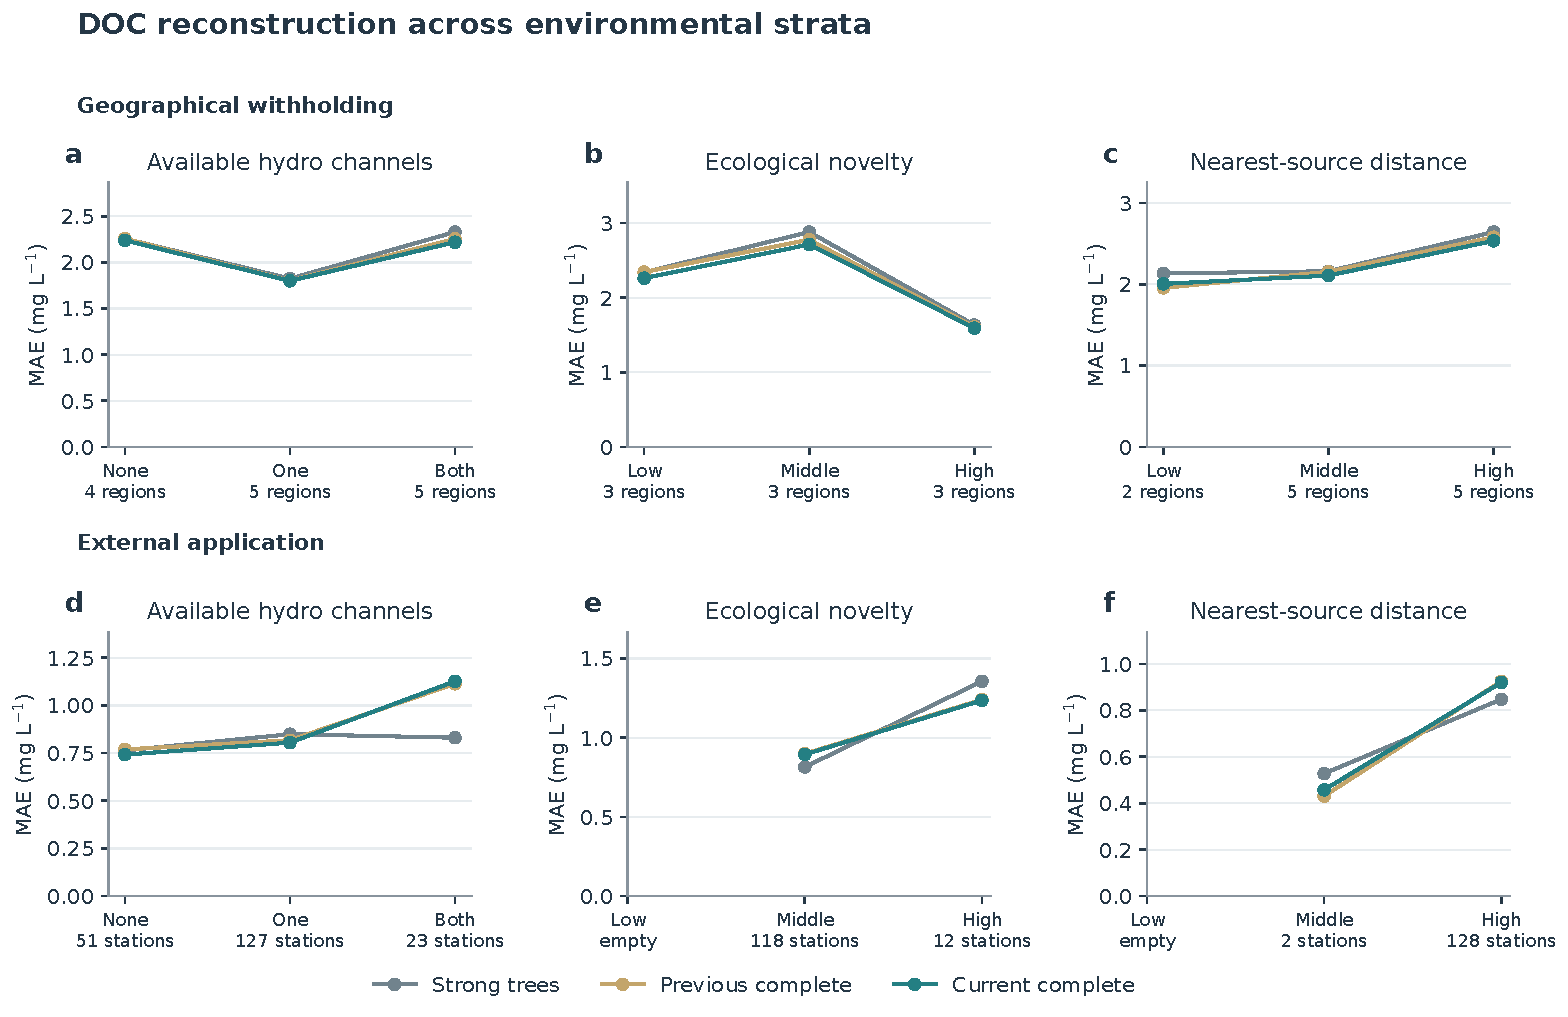
\includegraphics[width=\linewidth]{figures/spatiotemporal_v4/supp3_environment.pdf}
\caption{Environmental and hydrological strata from the evaluated current release, redrawn using the manuscript palette. Top panels use usable geographical region means; bottom panels use external ensemble cell errors. The original source-defined bins, station/region denominators and empty groups are retained.}
\end{figure}

Prior uncertainty studies remain a separate result. Validation-only recalibration repaired coverage with tool-dependent interval inflation, but the declared ranking criterion established monitoring value for only one of three tools. No stable blind-spot or active-sampling conclusion is added to this reconstruction manuscript.

\FloatBarrier
\section{Completed river and architecture explorations}
The main manuscript's fitted neural relation is source similarity. Completed real-upstream experiments are retained as development evidence. Their source-role partitions 142/143/144 and seeds 42/43/44 are not additional geographical or external confirmation.

On that development population, the complete predictor has MAE 1.723002~mg/L; observed-upstream attention has 1.717226; expanded upstream environmental state has 1.714729. The last comparison gives 0.480\% improvement over complete prediction [0.082,0.858\%]. Its matched real-upstream advantage over non-ancestor donors remains unresolved, and uniform allocation is slightly better than learned allocation. These values belong to the development task and cannot be substituted for the main geographical MAE.

Confluence mixing and storage gave no material new improvement. Actual source dates plus measured hydrological phase achieve 1.717288~mg/L, compared with 1.717226 for ordinary monthly attention: $-0.0036$\% gain [$-0.0443$,0.0337\%]. Source-age information alone changes error by approximately 0.004\%. These variants were not adopted in the released predictor. Further small extensions of the same readout are closed for this manuscript.

The morphology archive measures real upstream channel geometries and identifies 111 elongated tributary-rich, 33 mainstem-dominated sparse and 178 broad tributary-rich networks among 322 classified distinct networks. These describe continuous forms with nested drainage relationships. In the station-median DOC diagnostic, branch organization adds 5.59\% predictive information [2.02,8.42\%], conditional on the contextual features and model. This is a different endpoint from monthly DOC reconstruction.

The independent NEON form comparison contains thirteen sites in eleven upstream-overlap groups. Its primary branching comparison does not reproduce that improvement: $-2.08$\% [$-11.56$,6.59\%]. The predeclared subset with no shared ST357 upstream channels contains ten sites in eight groups and gives 13.32\% [1.48,32.41\%]. No elongated--broad pair meets the joint environmental matching criteria. Taken together, these results motivate branching-focused field work but do not establish a stable shape ordering or a general buffering effect. Controlled-routing and event studies are preserved separately from field reconstruction evidence.

Additional shared-analyte, chemistry-adaptation, deeper/residual graph, wider-source and source-state-key experiments remain archived. They are not presented as separate contributions of the consolidated DOC framework. The evidence ledger gives their placement and original study directories.

\section{Reproducible paper assembly}
From the repository root, run the following through the existing uv-managed environment:
\begin{verbatim}
uv run python scripts/consolidate_doc_spatiotemporal_v4.py
uv run python scripts/plot_doc_spatiotemporal_v4.py
\end{verbatim}
The first command independently recomputes point metrics from saved predictions, checks task populations, repeats fourteen primary paired contrasts with 5,000 draws and verifies agreement with the original analyses. It creates a unified result table, detailed metrics, fixed-query curves, source manifest and evidence ledger under \nolinkurl{docs/paper/doc_spatiotemporal_consolidation_v1/}. The second produces five core vector figures and supplementary diagnostics. Original prediction directories and manuscript version three remain intact. Compile the main and supplementary TeX files twice using the installed local TeX Live, then inspect their rendered pages.

\end{document}
